 \documentclass{article}
\usepackage[utf8]{inputenc}
\usepackage{graphicx}

\title{Mid level discriminative patches for facial expression recognition}
\author{Ioannis Papadopoulos }
%\date{December 2015}

\begin{document}

\maketitle

\setlength\parindent{0pt}

\section{Introduction}
There is a lot of ongoing research in the field of unsupervised image recognition. Most machine learning algorithms are not equipped to handle images at the raw pixel level. Some of the most popular image representations are based on extracting visual words introduced in \cite{words}. The term words is used as an analogy to the way text sentences are constructed from individual words. Visual words are a very low level representation, capturing local edges and corners \cite{mode}. 
\newline \newline
More recently, \cite{paris} obtained promising results using  mid level discriminative patches, a higher level representation. Figure \ref{fig:comparison} illustrates the patches most confidently detected by each approach. It can be argued that the top-left images are a more intuitive representation. Extending the analogy of visual words, these patches can be thought of as visual phrases. The goal of our research project was to apply the same technique to classify facial expressions according to emotions, such as happiness and anger.

\begin{figure}
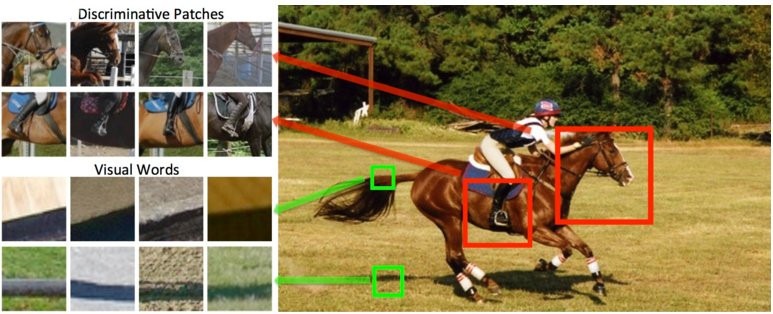
\includegraphics[width=400pt]{patches.jpg}
  \caption{Top visual words detected (bottom) vs Mid level discriminative patches}
  \label{fig:comparison}
\end{figure}

\section{Mid level discriminative patches}
A mid level discriminative patch is a section of an image which corresponds to an object or a feature of the image. The key requirements for patches are that they should be representative of the image and sufficiently different from other images to perform classification and detectable with high precision in a large number of images. These patches should be discovered in a fully unsupervised manner, using only the raw pixels as input. No extra context information may be given to the algorithm, for example that the areas around the eyes and mouth are often descriptive of the expression. 

\section{Algorithm}

The first key requirements for good discriminative patches – to occur frequently, is common to most other object discovery approaches. The
standard solution is to employ some form of unsupervised clustering, such as K-means. \cite{discr} showed that just using k means does not produce very good results because  unsupervised clustering
like k-means has no choice but to use a low-level distance metric (e.g. Euclidean) which does not work well for medium-sized patches, often combining instances which are not visually similar.
\newline \newline
However, given a set of patches were visually similar, we could easily train
a discriminative classifier, such as a linear support vector machine (SVM), to produce an appropriate similarity metric for these patches. This can be approached with iterative discriminative clustering. We start with an arbitrary initialization of the clusters. The iterative step consists of training an SVM classifier for each cluster, then re-assigning clusters according to the svm distance metric. Additionally, the images are divided into two equal non-overlapping sets, the training and the validation set. In the first step of the iteration the svm classifier is run on the training set while and k-means clustering on the validation set, then in each iteration the training and validation sets are swapped. After the clusters have converged the top patches according to the ranking described in the following subsection are returned as the algorithm's output. The pseudo code of the algorithm can be found in Figure \ref{fig:alg}.


\begin{figure}
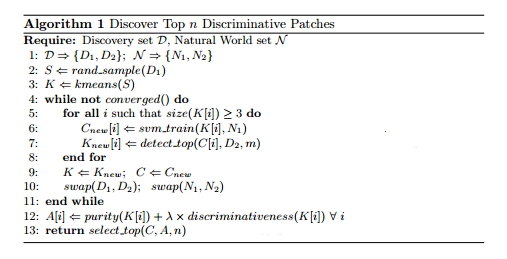
\includegraphics[width=300pt]{alg.png}
  \caption{Pseudocode of the algorithm}
  \label{fig:alg}
\end{figure}

\subsection{Ranking the patches}
The ranking for each linear is a linear combination of two factors: \newline 
Discriminativeness: The discriminativeness of a patch measures the ratio of the patch firing on images belonging to the same class, over firing on images belonging to all other clusters. \newline 
Purity: Typically in clustering algorithms purity would measure whether the patches in the same cluster all capture the same concept, e.g. the mouth when the person being depicted is smiling. In a fully unsupervised approach this is not possible, since the algorithm is given no such labelling as input. Instead, the purity is measured as the sum of the top svm detection scores of the cluster members.

\section{Image Dataset}
After browsing several databases of facial expressions the CK+ dataset \cite{ck} was chosen as most appropriate. It consists of 561 images of 8 different emotions: Neutral, Anger, Contempt, Digust, Fear, Happy, Sadness and Surprise. The facial images are all the same size, taken under similar lighting conditions and focused on the facial area.  These uniform standards somewhat simplify the classification task. The images were converted to gray scale. The color information is not especially helpful for classification, and a single color channel significantly reduces the dimensionality of the feature space 

\section{Results}
As an intermediate step of our research project before fully unsupervised classification we decided to skip the clustering step. Instead we manually extracted the most likely patches and focused on the classification step. Early results showed that some of the expressions such as surprise and anger are detected with high precision. There were more classification errors for subtler expressions like contempt.

\section{Future work}
Several standard image processing and machine learning techniques can be applied in order to improve the quality of the results. Images can be preprocessed to normalize contrast and lightning conditions. Additionally, the classifier would likely perform better with a larger dataset of images. It is however difficult to find more images of the same quality following the same uniform standards. As an alternative, the original images can be distorted or flipped along the y-axis to create additional instances. 
\newline \newline
After we've obtained satisfactory results for the classification we'll proceed with fully unsupervised detection with the iterative algorithm described in Section 3. An extendable framework will be created to enable additional research on the topic.


\section{Conclusion}
The results obtained so far indicate that mid-level discriminative patches can be applied to classifying facial expressions. It has not yet been established if the fully unsupervised approach can lead to good results. Demonstrating this will require additional work on the preprocessing steps and possibly combining other machine learning techniques. 

\bibliographystyle{apalike}
\bibliography{references}

\end{document}

